\pagebreak
\section{Identifikation der Reaktionsprodukte}

Die Produkte der Reaktion mit Essigsäureanhydrid konnten ebenfalls mithilfe von \gls{lcms} identifiziert werden. In Abbildung \ref{fig:HPLCChromatogrammRP} sind die Reaktionsprodukte, die mittels Online-UV/Vis Spektren identifiziert wurden, dargestellt. Die dazugehörigen UV/Vis Spektren werden in Abbildungen \ref{fig:YCC3398}-e dargestellt. Es handelt sich dabei um die Hauptreaktionsprodukte, die in der \gls{hplc} dadurch charakterisiert sind, dass sich ihre Retentionszeiten nach hinten verschieben. Sie dürften somit apolarere Eigenschaften besitzen wie die \gls{Chl-K}en, was vermutlich durch den Methylester bedingt ist. Über die Verschiebung der Peaks im \gls{hplc} Chromatogramm wird das Stattfinden der Reaktion auf einen Blick ersichtlich (vergleiche Abbildung \ref{fig:HPLCChromatogramm} und Abbildung \ref{fig:HPLCChromatogrammRP}). Zudem konnten im Vergleich zu den \gls{hplc} Läufen ohne Reaktion mehr Verbindungen über Online-UV/Vis Spektren beobachtet und identifiziert werden, da es zu einer größeren Auftrennung kommt.

\begin{figure}[!htbp]
  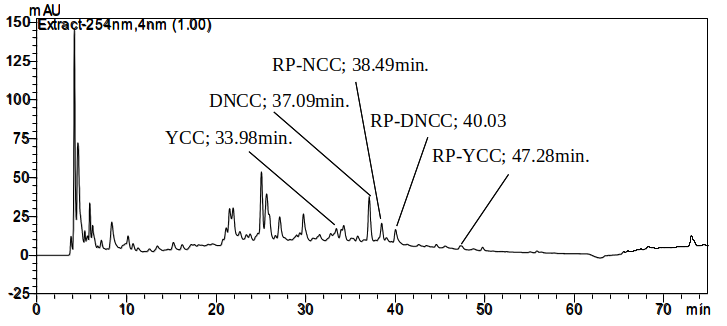
\includegraphics[width=\textwidth]{figures/Kapitel6/Reaktion3h/HPLC_Chromatogramm.png}
  \caption[HPLC Chromatogramm nach 3h Reaktionsdauer, Quelle: Autor]{\gls{hplc} Chromatogramm, gefunden wurden Reaktionsprodukte mit den Eigenschaften eines NCCs (RT = 38.49min.), eines DNCCs (RT = 40.03min.), eines YCCs (RT = 47.28min.) und eines weiteren DNCCs (37.09min.); beim YCC bei RT = 33.98min. könnte es sich um einen weiteren \gls{Chl-K}en handeln}
  \label{fig:HPLCChromatogrammRP}
\end{figure}

Das Chromatogramm des Massenspektrometers des \gls{lcms} Laufes (Abbildung \ref{fig:LCMSCChromatogrammRP}) zeigt die Massen aller \gls{Chl-K}en und die Zeitpunkte, zu denen sie jeweils eluieren. Durch die stattgefundene Reaktion sind dementsprechend mehr Signale vorhanden. Zu beachten ist, dass aufgrund der Aufarbeitung mit \gls{meoh} nicht ein Essigsäureanhydrid beobachtet wird, sondern der Methylester, der sich offensichtlich aufgrund der vermeintlich guten Abgangsgruppe \ch{CH3COOH} schnell bildet (auch Kapitel \ref{sec:ChlKatabolitenBrokkoli} und \ref{sec:RPMSLeafspray}). \\

Auffallend ist, dass manche Verbindungen in ihren Retentionszeiten verschoben worden sind. So eluiert Verbindung mit m/z = 631 [M+H]\textsuperscript{+} nun bei 39.0min. im Vergleich zu 18.9min., Verbindung mit m/z = 629 [M+H]\textsuperscript{+} bei 31.8min. im Vergleich zu 21.6min. und Verbindung mit m/z = 645 [M+H]\textsuperscript{+} bei 34.5min. im Vergleich zu 29.0min. (vergleiche Abbildungen \ref{fig:LCMSCChromatogrammRP} und \ref{fig:LCMSChromatogramm}). Gründe für diese Verschiebungen müssten weiter untersucht werden bzw. müsste überprüft werden, ob es bei den Versuchen, aus denen einer zu Abbildung \ref{fig:LCMSChromatogramm} führte, nicht einen Messfehler gab. Eine Überprüfung und erneute Durchführung der Messung im Rahmen meiner Vorwissenschaftlichen Arbeit führte zum selben Ergebnis (siehe Anhang). 

\begin{figure}[!htbp]
  \centering
  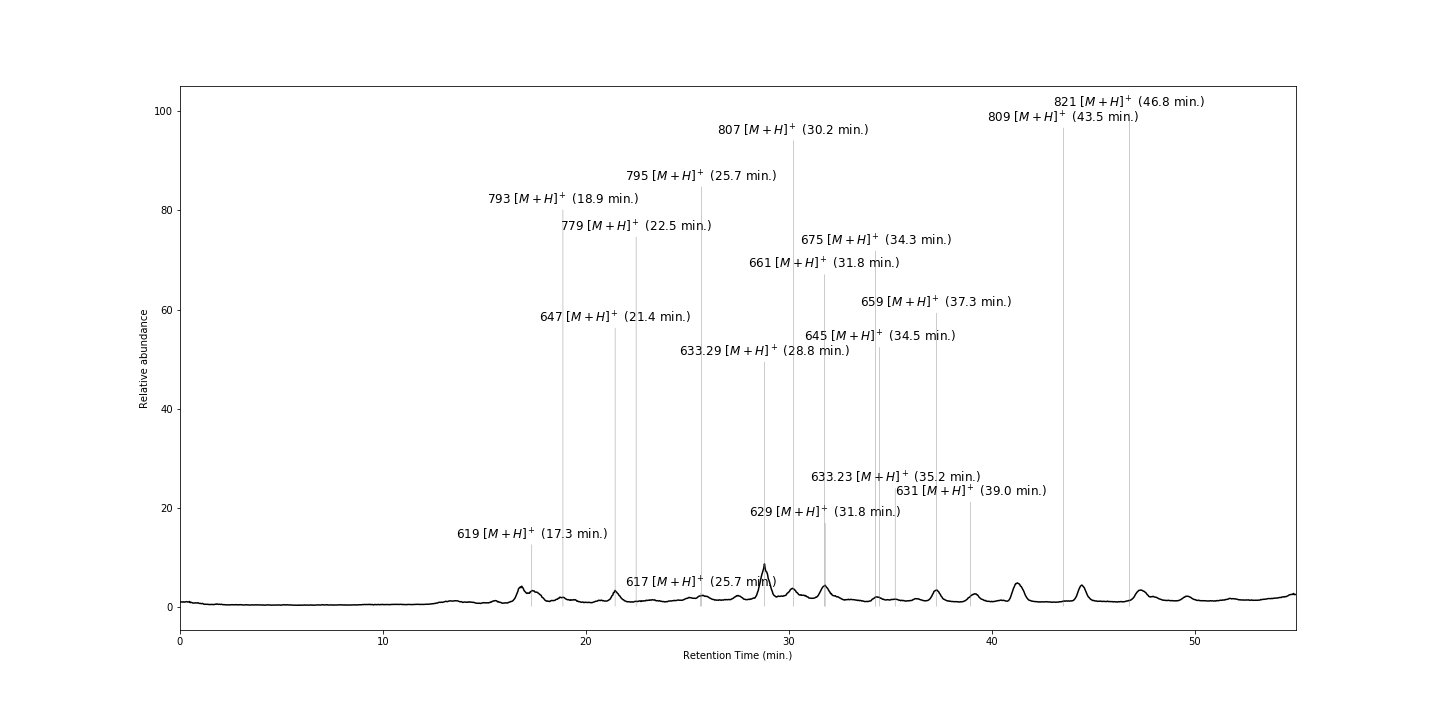
\includegraphics[width=1.4\textwidth, center]{figures/Kapitel6/Reaktion3h/Kuerbis_Analyse_Reaktion3h_Ganzes_Spektrum.png}
  \caption[LC-MS Chromatogramm nach 3h Reaktionsdauer, Quelle: Autor]{\gls{lcms} Chromatogramm}
  \label{fig:LCMSCChromatogrammRP}
\end{figure}

In Tabelle \ref{tab:LCMSKatabolitenRP} werden die \gls{Chl-K}en dargestellt, die nach der Reaktion gefunden wurden. Dabei wurde neben dem erwarteten Reaktionsprodukt bei m/z = 659.2741 [M+H]\textsuperscript{+} eine weitere Verbindung bei m/z = 659.2348 [M+H?]\textsuperscript{+} entdeckt, jedoch mit einer anderen Summenformel. Wie dieses Signal zustandekommt bleibt ungeklärt. Da bei m/z = 633 [M+H]\textsuperscript{+} ebenfalls zwei Molekülmassen beobachtet wurden (m/z = 633.2955 und m/z = 633.2339), könnte es sich um ähnliche Charakteristiken handeln, die jedoch weiter untersucht werden müssten. Von einer anderen Verbindungsklasse ist aufgrund der passenden Summenformel mit entsprechender Doppelbindungsäquivalenz und dem Massendefekt nicht auszugehen! \\

In Abbildung \ref{fig:LCMSChromatogrammRPAufspaltung} wird nur unter Verwendung von Massenspektrometerdaten ersichtlich, dass die Reaktion stattgefunden hat. Es wird angenommen, dass die Peakhöhen in direkt proportionaler Abhängigkeit mit der quantitativen Anzahl der jeweiligen Ionen steht.

Man sieht, dass die Intensität des Bo-DNCC zurückgegangen ist, wohingegen jene von m/z = 633 [M+H]\textsuperscript{+}, dem Reaktionsprodukt viel größer ist. Ähnliche Verschiebungen sind von Bo-NCC-1 auf m/z = 807 [M+H]\textsuperscript{+} und 821 [M+H]\textsuperscript{+} sowie von Bo-NCC-3 auf m/z = 661 [M+H]\textsuperscript{+} und 675 [M+H]\textsuperscript{+} sichtbar. Die anderen Intensitätsverschiebungen sind nicht so groß, dass sie in diesem Kontext interpretierbar wären. Sie sind aber trotzdem vorhanden.

\begin{figure}[!htbp]
  \centering
  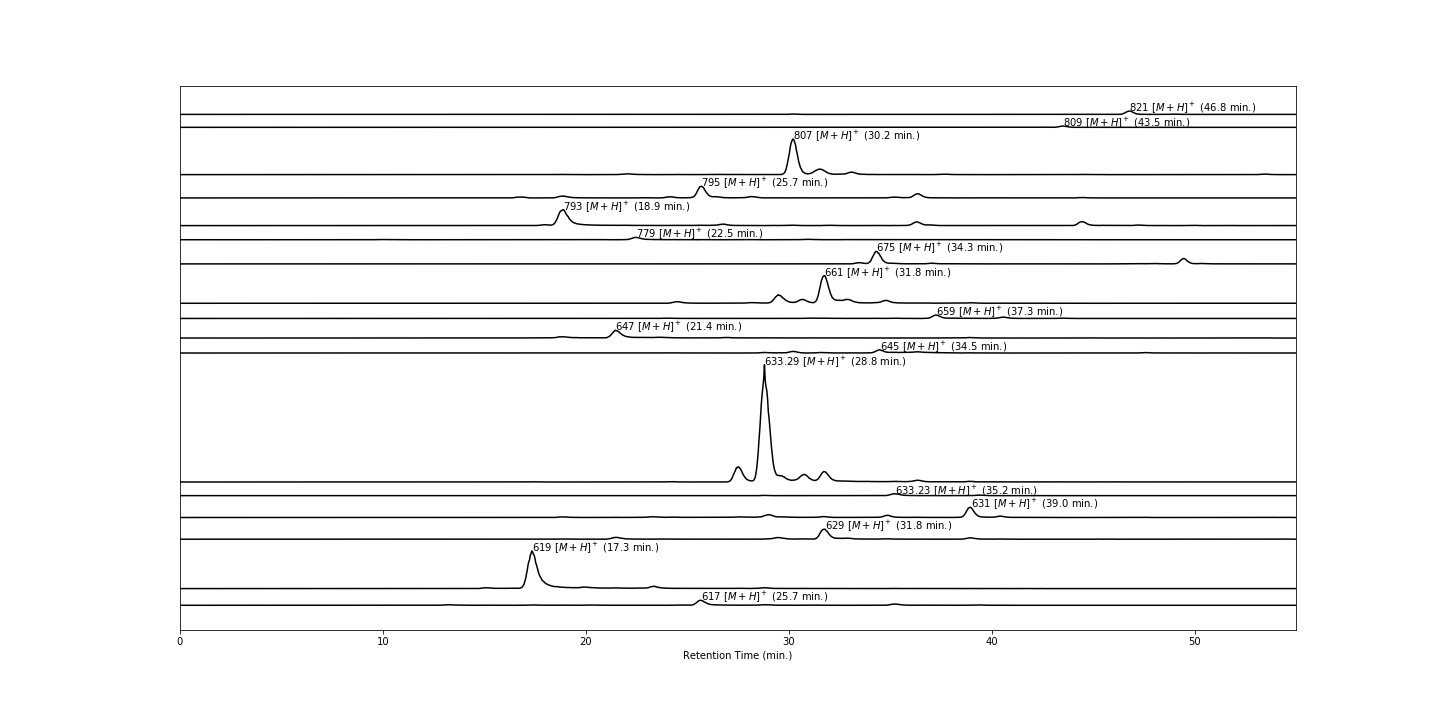
\includegraphics[width=1.4\textwidth, center]{figures/Kapitel6/Reaktion3h/Kuerbis_Analyse_Reaktion3h_LC-ESI-MS.png}
  \caption[LC-MS Chromatogramm nach 3h Reaktionsdauer - Aufspaltung, Quelle: Autor]{\gls{lcms} Chromatogramm}
  \label{fig:LCMSChromatogrammRPAufspaltung}
\end{figure}

Um das Stattfinden der Reaktion zu sehen, vergleiche mit Abbildung \ref{fig:LCMSChromatogrammAufspaltung}.

\begin{table*}[!htbp]\centering
  \ra{1.3}

  \begin{tabular}{cccccc}\toprule
 Bezeichnung & Summenformel & M (in Da) & Typ & RT\textsubscript{HPLC} (in min.) & H. \\
\midrule
\rowcolor{black!20} Bo-DYCC & \ch{C33H37O8N4} & 617.2599 & DYCC & 30.94? & - \\
 Bo-DNCC & \ch{C33H39O8N4} & 619.2798 & DNCC & 26.72 & - \\ 
\rowcolor{black!20} • & \ch{C34H37O8N4} & 629.2641 & • & - & - \\ 
 - & \ch{C34H39O8N4} & 631.2795 & DYCC & 29.91, 30.94 & Bo-DYCC \\ 
\rowcolor{black!20} - & \ch{C34H41O8N4} & 633.2955 & DNCC & 28.8 & Bo-DNCC \\ 
 • & \ch{C36H33O7N4} & 633.2339 & • & - & - \\ 
\rowcolor{black!20} Bo-YCC & \ch{C34H37O9N4} & 645.2593 & YCC & - & - \\ 
 - & \ch{C35H41O8N4} & 645.2953 & DYCC & - & Bo-DYCC \\ 
\rowcolor{black!20} Bo-NCC-3 & \ch{C34H39O9N4} & 647.2748 & NCC & 33.04 & - \\ 
 • & \ch{C34H35O10N4} & 659.2348 & • & - & - \\
\rowcolor{black!20} - & \ch{C35H39O9N4} & 659.2741 & YCC & 37.09 & Bo-YCC \\
 - & \ch{C35H41O9N4} & 661.2902 & - & - & Bo-NCC-3 \\
\rowcolor{black!20} - & \ch{C36H43O9N4} & 675.306 & - & - & Bo-NCC-3 \\
 Bo-DNCC-2 & \ch{C39H47O13N4} & 779.3181 & DNCC & - & - \\ 
\rowcolor{black!20} Bo-NCC-1 & \ch{C40H49O13N4} & 793.3336 & NCC & 29.91 & - \\ 
 - & \ch{C40H51O13N4} & 795.3491 & - & - & - \\ 
\rowcolor{black!20} - & \ch{C41H51O13N4} & 807.3491 & NCC & 40.03 & Bo-NCC-1 \\ 
 - & \ch{C41H53O13N4} & 809.3649 & - & - & 795 \\ 
\rowcolor{black!20} - & \ch{C42H53O13N4} & 821.3652 & NCC & 47.28 & Bo-NCC-1 \\ 
\bottomrule
  \end{tabular}
  \caption[Übersicht über die Chl-Kataboliten des Brokkoliblattes, Quelle: Autor]{Übersicht über die gefundenen Chl-Kataboliten des Brokkoliblattes und ihren Methylestern, die sich aus der Reaktion der freien Carbonsäure mit Essigsäureanhydrid und der anschließenden Aufarbeitung mit \gls{meoh} ergeben. Durch die Aktivierung der Reaktion durch Essigsäureanhydrid sind mehr Produkte zu sehen und diese sind in größeren Intensitäten vorhanden. (die Summenformeln und die exakten Molekülmassen beziehen sich auf die [M+H]\textsuperscript{+} Ionen)}
  \label{tab:LCMSKatabolitenRP}
\end{table*}

\pagebreak
Mithilfe von UV/Vis Spektren konnten ein YCC (RT = 33.98min.), ein DNCC (RT = 37.09min.), ein NCC (RT = 38.94min.), ein weiterer DNCC (RT = 40.03min.) und ein YCC (RT = 47.28min.) identifiziert werden (Abbildungen \ref{fig:YCC3398}-e). 

\begin{figure}[!htbp]
  \begin{subfigure}[b]{0.5\textwidth}
    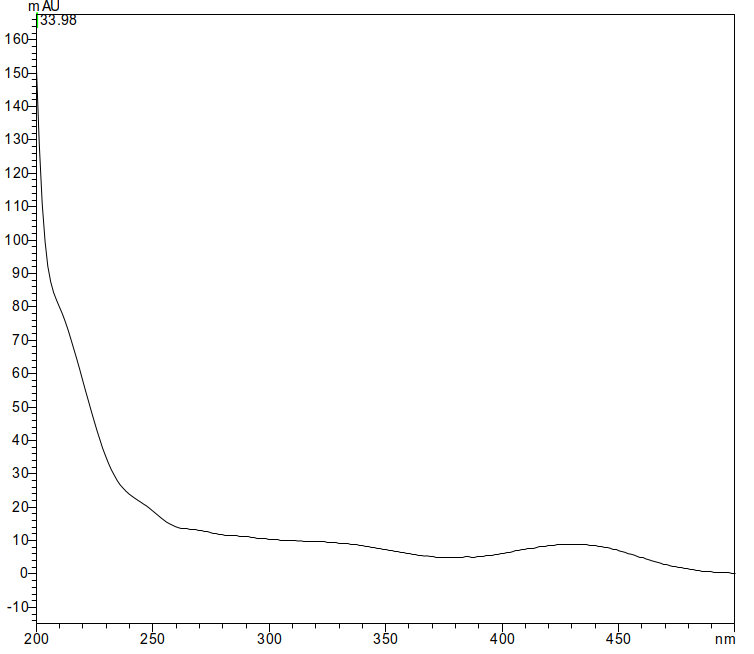
\includegraphics[width=\textwidth]{figures/Kapitel6/Reaktion3h/YCC3398.png}
    \caption{}
    \label{fig:YCC3398}
  \end{subfigure}
  \hfill
  \begin{subfigure}[b]{0.5\textwidth}
    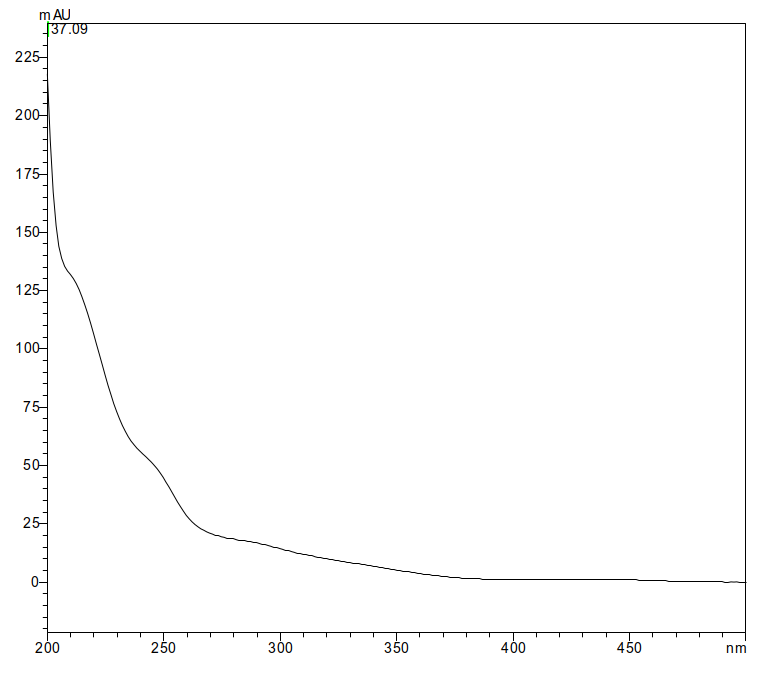
\includegraphics[width=\textwidth]{figures/Kapitel6/Reaktion3h/DNCC3709.png}
    \caption{}
    \label{fig:DNCC3709}
  \end{subfigure}
  
  \begin{subfigure}[b]{0.5\textwidth}
    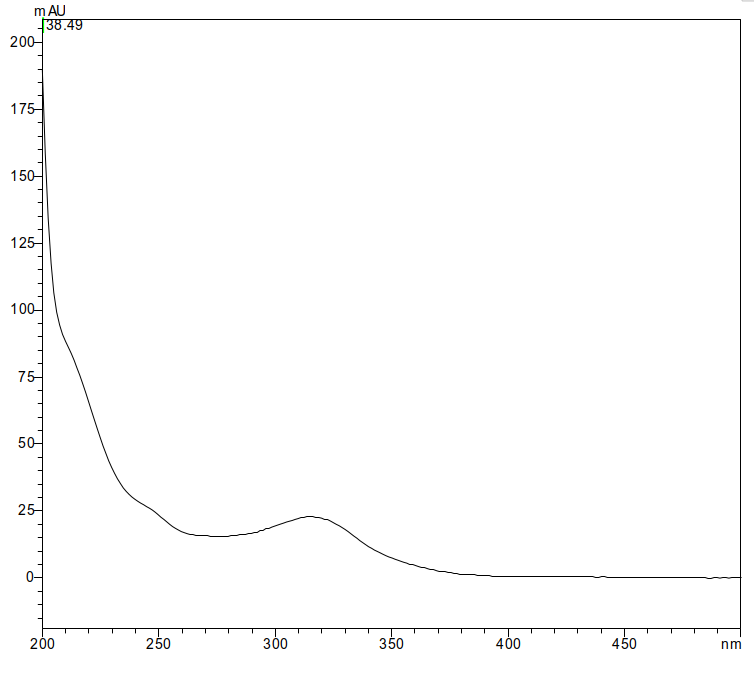
\includegraphics[width=\textwidth]{figures/Kapitel6/Reaktion3h/NCC3849.png}
    \caption{}
    \label{fig:NCC3849}
  \end{subfigure}
  \hfill
  \begin{subfigure}[b]{0.5\textwidth}
    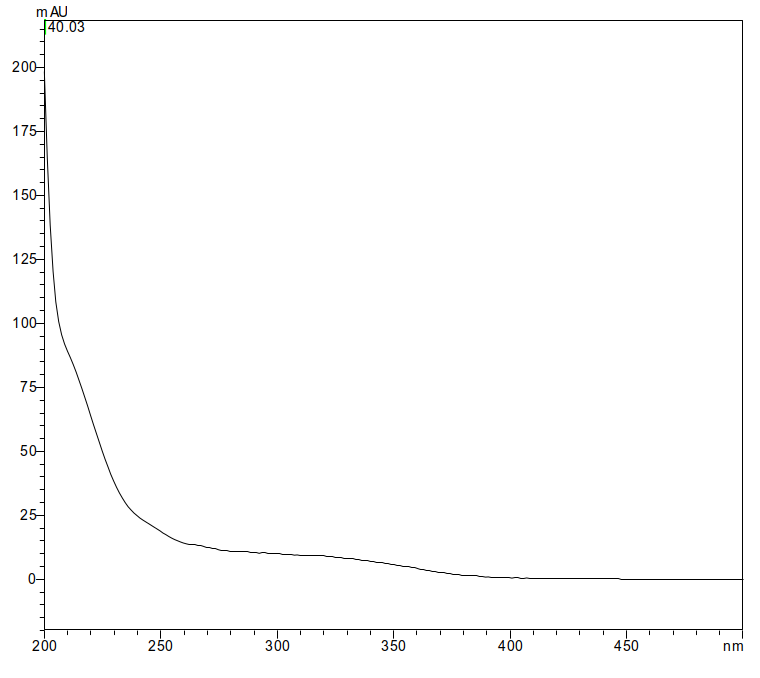
\includegraphics[width=\textwidth]{figures/Kapitel6/Reaktion3h/DNCC4003.png}
    \caption{}
    \label{fig:DNCC4003}
  \end{subfigure}
  \caption[Online-UV/Vis Spektren mit der Charakteristik eines YCC bei 33.98min., eines DNCC bei 37.09min. eines NCC bei 38.94min. sowie eines DNCC bei 40.03min., Quelle: Autor]{Online-UV/Vis Spektren: charakeristisch für (a) \gls{YCC} - RT = 33.98min., (b) \gls{DNCC} - RT = 37.09min., (c) \gls{NCC} - RT = 38.94min., (d) \gls{DNCC} - RT = 40.03min., (e) \gls{YCC} - RT = 47.28min.}
\end{figure}

\begin{figure}[!htbp]
  \centering
  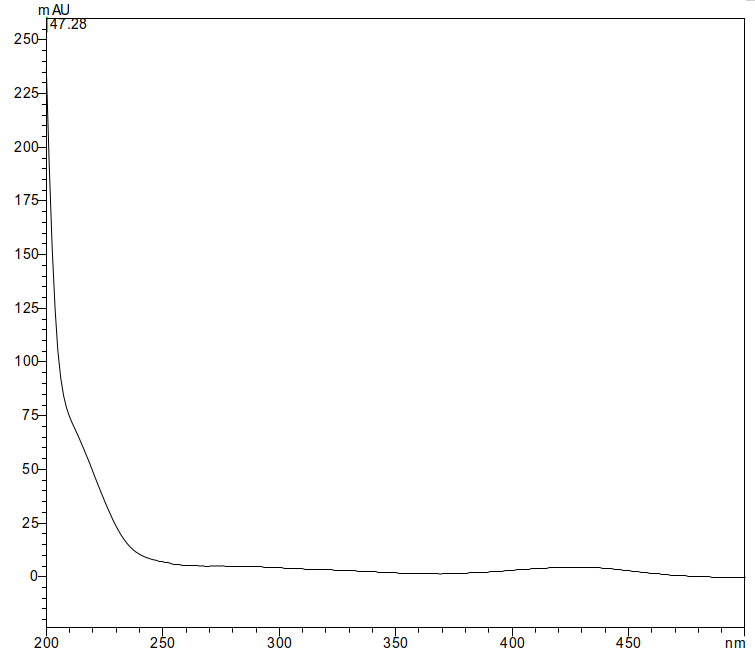
\includegraphics[width=0.5\textwidth]{figures/Kapitel6/Reaktion3h/YCC4728.png}
  \caption{}
  \label{fig:YCC4728}
  \caption[Online-UV/Vis Spektren mit der Charakteristik eines YCC bei 47.28min., Quelle: Autor]{Online-UV/Vis Spektrum charakteristisch für einen  \gls{YCC} - RT = 47.28min.}
\end{figure}

